We will make our quantum array out of neutral strontium atoms. The tool to cool, trap and move these atoms is light. We need individual control for this. In 2001, a group from Paris showed for the first time, that if you tune your tweezer in the right way, it's possible to trap single atoms.         


 
\section{High NA objective}

In order to trap single atoms, we need to make the smallest possible spot size, the diffraction-limited spot. Fourier optics tells us that in order to make the smallest possible spot, we want to focus the light using the largest possible cone of light, so we need high NA. Apart from high NA we also need ultralong working distance, because the lens will be positioned outside of the vacuum. 

We chose the G Plan Apo 50X microscope objective from Mitutoyo. It has a fairly high NA of 0.5 and is corrected for spherical aberrations as a result of imaging through a 3.5 mm glass plate, which we will use for our vacuum. The exact glass material is not specified but we have assumed it to be N-KB7. It is designed for a finite conjugate and has a back aperture of 4 mm. We will now estimate how we use this objective in our setup. 

\subsection{Intermezzo Fourier Optics}

As we use the objective to make a tweezer, light is impinging on its back aperture. We call its complex amplitude $U(x',y')$ and define the aperture at $z = 0$ on the optical axis. After the aperture, light will show diffraction. An elegant description is provided by scalar diffraction theory. We will not repeat a full derivation here but we can refer the reader to \cite{Goodman2005}.Consider the Fresnel diffracion integral in cartesian coordinates. After the aperture, the complex amplitude $U$ distribution is:

\begin{equation}\label{FresnelDiffraction}
    U(x,y,z) = 
    \frac{e^{ikz}}{i \lambda z} \iint_{-\infty}^{\infty} U(x',y',0) \exp{\frac{ik}{2z}} \exp{\left[(x-x')^2+(y-y')^2\right]} dx'dy'.
\end{equation}

In \cref{FresnelDiffraction}, $\lambda$ is the wavelength, $k=2\pi/\lambda$ the wavenumber. In this thesis, we are usually not immediately interested in describing the light in the the near field of the aperture, but in the far-field. More formally, the following needs to apply:

\begin{equation}\label{FraunhoferCriterion}
    z \gg k R^2/2,
\end{equation}

where $R$ is the maximum distance from the aperture to the optical axis. While this criterion is in practice not met, it does hold in the focal point of a lens, because a lens projects an image in infinity to its focal length $f$. Inserting \cref{FraunhoferCriterion} in \cref{FraunhoferDiffraction} yields:

\begin{equation}\label{FraunhoferDiffraction}
    U(x, y, z)=\frac{e^{i k z} e^{i k\left(x^{2}+y^{2}\right)/2}}{i \lambda z} \iint_{-\infty}^{\infty} U(x', y') \exp \left[\frac{-ik}{z}(x x'+y y')\right] dx' dy'
\end{equation}. 

We recognize in \cref{FraunhoferDiffraction} the spatial Fourier transform, in both $x$ and $y$ with respectively the frequencies $f_x = x/\lambda z$ and $f_y = y/\lambda z$. \cref{FraunhoferDiffraction} is the Fraunhofer diffraction integral, it will be used later in this work as well. Returning back to our aperture, we are concerned with a circular aperture so a switch to cylindrical coordinates seems natural. Ignoring the phase factor in front of the integral:

\begin{equation}\label{FraunhoferRTheta}
    U(r,\theta, z) \propto \iint U(r') \exp{(\frac{- i k rr'}{z})} \exp{\left(\cos{(\theta-\theta')}\right)} r'dr'd\theta'.
\end{equation}

Using the integral definition of the Bessel function of the first kind\footnote{$J_0(x) = \frac{1}{2\pi} \int_0^{2\pi} \exp{(i x \cos{\alpha})} d\alpha$} we write \cref{FraunhoferRTheta} as 

\begin{equation}\label{FourierBessel}
    U(r,z) \propto 2\pi \int_0^{\infty} U(r') J_0\left( \frac{k r r'}{z}\right) r'dr'
\end{equation}

\cref{FourierBessel} is the Fourier-Bessel or Hankel transform. 

\subsection{Circular aperture}

Returning to initial problem: we send a Gaussian beam with width $w_i$ through an aperture of radius $R$ and are interested in what happens in the focal plane of a lens $z\approx f$

\begin{equation}\label{FourierBesselAperture}
    U(r) \propto \int_0^R e^{-r'^2/w_i^2} J_0\left(\frac{k r r'}{f}\right)r'dr'
\end{equation}

This integral has no analytical solution. We can however find an expression for the power transmission of a Gaussian beam with width $w_i$ sent through a circular aperture with radius $R$, the fraction of power transmitted issue

\begin{equation}\label{FracPowerCircular}
    P/P_0 = 1 - e^{-w_i^2/R^2}
\end{equation}

We follow \cite{Madjarov2021} and look at two extreme cases for \cref{FourierBesselAperture,FracPowerCircular}

\begin{enumerate}
    \item $w_i \gg R$. \cref{FracPowerCircular} tells us we lose almost all of our power. The aperture function can be approximated by a plane wave and dropping the exponential term in \cref{FourierBesselAperture} we find
    \begin{equation}\label{Airy}
        U(r) \propto \frac{f}{k r} J_1\left(\frac{k r R}{f}\right)
    \end{equation}
    which is the equation for an Airy pattern. It is the smallest feature a lens can produce. 

    \item $w_i \ll R$. The waist is much smaller than the aperture, according to \cref{FracPowerCircular} we have maximum power efficiency. We let the integration boundary run to infinity and using a Hankel tranform pair\footnote{$F_0(k) = \int_0^{\infty} e^{-1/2 a^2 r^2} J_0(k r)r dr = \frac{1}{a^2} e^{-\frac{k^2}{2a^2}}$} find 
        \begin{equation}
        U(r) \propto \frac{w_i^2}{2} \exp{\left(\frac{-k^2w_i^2 r^2}{2f^2}\right)}.
    \end{equation}
    The result is a Gaussian, but with a modified waist of $\lambdaup f / \pi w_0$.  The result is similar to Gaussian apodization, where the size lobes of the Airy function are gone. 
\end{enumerate}

\section{Tweezer potential}

Because we are interested mostly in what happens near the deepest point of the trap, we model the optical dipole trap as a gaussian with a maximum trap depth $-U_0$, waist $w_0$ and Rayleigh range $z_R$ to find 

\begin{equation}\label{GaussianPotential}
    I(r,z)=\frac{-I_{0}}{1+z^{2} / z_{R}^{2}} \exp \left(\frac{-2 r^{2}}{w_{0}^{2}\left(1+z^{2} / z_{R}^{2}\right)}\right)
\end{equation}

We can discuss the two extreme cases again:

\begin{enumerate}
    \item For the case $w_i \gg R$, the power transmission will be low and therefore also the trap depth $-U_0$.
    \item For $w_i \ll R$, the waist of the resulting Gaussian in radial and longitudal directions $w_0$ and $z_R$ will increase, which is undesired. Because the total amount of power in the trap is fixed, because of normalization the trap depth is lower as well. 
\end{enumerate}

It is clear that the optimum is somewhere in between these two extreme cases.  

The atoms will spend most of their time in the bottom of the tweezer. \cref{GaussianPotential} can be tailorexpanded in around the center of the tweezer, or $(r,z) = (0,0)$.

\begin{equation}\label{TaylorGaussianPotential}
    I(r,z) \approx I_0 \left(1 - \frac{2r^2}{w_0^2} - \frac{2z^2}{z_R^2}\right) \quad \text{at} \quad (r,z) = (0,0)
\end{equation}

For a potential of the form \cref{TaylorGaussianPotential} we know the frequencies: we can define the radial and longitudinal trap frequencies $\omega_r = 2\left(U_0/m w_0^2\right)^{1/2}$ and $\omega_z= \left(2 U_0/m z_R^2\right)^{1/2}$. Because we want a narrow and deep tweezer, the higher the trap frequency the better. 

The optimum trap frequency was computed numerically by \cite{Madjarov2021} and was found to be $w_i \approx R$. We will apply this result experimentally. 


\section{Point Spread Function and Diffraction Limit}

Because of the wave nature, we cannot focus a laser beam to an infinitely small spot. The smallest possible feature our high NA objective can produce is the point spread function (PSF), which we have seen is the result of illuminating the objective with a plane wave. Using \cref{Airy} we find for the intensity of the PSF around the focused beam waist:

\begin{equation}\label{AiryIntensity}
    I(r) \propto \left[\frac{J_1(krR/f)}{krR/f} \right]^2
\end{equation}

Solving for the first minimum of \cref{AiryIntensity}, we will call this radius $d$:

\begin{equation}\label{Abbe}
    d = 0.61 \frac{\lambdaup}{\text{NA}}
\end{equation}

This result is known as the Abbe limit \cite{Hecht2002} and is the reason we want to use an objective with the highest possible NA, it is Because we will not be illuminating the objective with a plane wave, but with a gaussian with a similar waist as the aperture radius, we will recover a pattern between a Gaussian and an Airy disk. It will turn out the pattern can be fit extremely well by a Gaussian ($R^2 > 0.99$). Fitting a Gaussian to an Airy disk, we find for the waist

\begin{equation}\label{GaussianAiryFit}
    w = 0.42 \frac{\lambdaup}{\text{NA}}
\end{equation}
 
Thus, when we fit a Gaussian to an Airy pattern, we can find the diffracion-limited waist from \cref{Abbe} as $w \approx 0.69 d$. Because we will use $\lambdaup = 780$ nm and $\text{NA}=0.5$ our diffraction-limited waist is $w = 655$ nm. If our waist is at this limit, we say the system is diffraction-limited, that is limited by the wave nature of light and not by aberrations or imperfections in the system. 


\section{Measuring the Tweezer potential}

We would like to measure tweezer potential of our high NA objective. We could use the objective to look at a pinhole and record its point spread function. However, in practice we don not send a plane wave but a Gaussian beam through the objective. As a result of this, two things are different \cite{Sortais2007}

\begin{itemize}
    \item As a result of apodization, the Airy rings will be damped. 
    \item The tweezer waist will be slightly broader: $\approx 9\%$.
\end{itemize}

In order to experimentally determine these effects, we send a Gaussian beam with a waist equal to the aperture radius through the microscope objective. We follow \cite{Baumgaertner2017}: we use another microscope objective to look into the tweezer waist of the Mitutoyo. But in order to avoid further convolution with the point spread function of the second objective, we use a higher NA for the second objective \footnote{Newport M-60X 0.85 NA objective}. Because there is no glass cell, this objective does not need ultra-long working distance so this higher NA is no problem. In order to record the 3D PSF, the tweezer is moved using a picomotor attenuator. 

\subsection{Calibration Imaging System}

The magnification of the Newport objective of 60X is only specified when used in a microscope with standard tube length distance, because it is finite conjugate corrected. Because our CCD is not exactly at the distance where normally the eyepiece of the microscope would be, we have to calibrate its magnification. We do this using a high resolution target \footnote{Edmund Optics high resolution microscope target.} 

We illuminate the target with an incoherent light source (LED) because the laser would cause interference from the different lines. We neglect the slightly different focus point from the Newport objective for our laser frequency compared to white light. 

\begin{figure}
    \centering
    \includegraphics[width = 2.5in]{figures/linespacing.pdf}
    \caption{Image from the resolution target illuminated showing lines spaced by 45 lines per mm.}
    \label{fig:resolutionTarget}
\end{figure}

To detect the edges in \cref{fig:resolutionTarget}, we use an edge detection algorithm script that averages over all vertical pixels, blurs using a Gaussian to surpress noise and computes the derivative. When the derivative surpasses a set threshhold we define it as an edge. The magnification was found to be $(50.3\pm0.5)$X. This is smaller than the specified 60X, which we attribute to an incorrect tube length distance. 

\subsection{Picomotor Attenuators}

The target was also used to calibrate the picomotor attenuator. We measured over the maximum available amount of lines of similar spacing of 5 using 4000 picomotor steps, and correcting for the shift in camera found a step size of $20.3\pm0.1$ nm, which matched exactly with the specifications of the piezo-attenuator for the given load. This result will be used in the 3D scanning of the tweezers. 

The stage we used is 8081-M 5-axis motorized tilt aligner from Newport. There is no reason here to use a 5-axis stage because we only need translation in one direction, but we will use this stage later to mount the objective in the final setup. To drive this stage, we used a set of Newport 8742 controllers in daisy-chain configuration. 


\section{Gaussian Beams}\label{sec:GaussianBeams}

Optical tweezer are in essence tightly focused laser beams. We will briefly revisit the description of the commonly used laser beam because it is used throughout this work. Starting from Maxwell equations, one can derive under paraxial approximation a description of the transverse electromagnetic mode (TEM\textsubscript{00}) \cite{Leeuwen2017} for the electric field $E$. This Gaussian beam is most conveniently written down in cylindrical coordinates $\{r,z\}$:

\begin{equation}\label{GaussianBeam}
	E(r,z) = \frac{w_0}{w(z)} \exp{\left(\frac{-r^2}{w^2(z)}\right)} \exp{\left[-ikz-i\frac{kr^2}{2R(z)} - i\psi(z)\right]},
\end{equation}

with parameters

\begin{equation}
	k = \frac{2\pi}{\lambdaup}, \quad 
	w(z) = \sqrt{w_0 + \frac{z^2}{z_R^2}}, \quad \text{and} \quad
	R(z) = z \left(1 + \frac{z^2}{z_R^2}\right).
\end{equation}

Respectively, the wave number in terms of the wavelength $\lambdaup$, the beam waist, the radius where the field drops $1/e$ in terms of $w(z)\equiv w_0$ and $R(z)$ is the wavefront curvature. Finally $\psi(z)$ is an extra phase term originating from the curvature of the wavefront known as the Gouy phase. We find the intensity of the Gaussian beam by taking the absolute value squared:

\begin{equation}\label{GaussianBeamIntensity}
	I(r,z) = I_0 \frac{w_0^2}{w^2(z)} \exp{\left(\frac{-2r^2}{w^2(z)}\right)}
\end{equation}

A sketch of a Gaussian beam profile is given in \cref{fig:GaussianBeam}, showing the $1/e$ field radius, or $1/e^2$ intensity radius $w_0$ and the Rayleigh range or depth of focus $z_R$. 

\begin{figure}
	\centering
	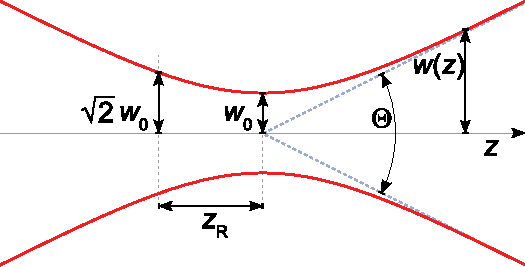
\includegraphics[width=0.4\linewidth]{figures/GaussianBeam.pdf}
	\caption{Gaussian beam profile and some key parameters used in this work, the beam waist $w_0$ and Rayleigh range $z_R$. Figure adapted from \cite{Hermans2009}.}
	\label{fig:GaussianBeam}
\end{figure}


\section{Loading Single Atoms}\label{sec:LoadingAtoms}

For the quantum register, an array of single atoms is needed. In order to do this, individual atoms from the cold atom cloud are loaded in optical tweezers, or tightly focused laser beams. We can write the dynamics of the number of atoms $N$ in the tweezer as \cite{Schlosser2002}

\begin{equation}\label{LoadingTweezer}
	\frac{\text{d}N}{\text{d}t} = \alpha - \gamma N - \beta N(N-1)
\end{equation}

where the first term $\alpha$ is the loading rate or the amount of Rb atoms entering the tweezer per second. Next, $\gamma$ is the atom loss as a result of collisions with the background gas. Lastly, $\gamma$ is a measure for the mainly 2 body loss as a result of light-assisted collisions. No additional laser is required for this, the MOT beams can be used for this purpose.  

We are interested in the case $\beta \gg \gamma$: the two-body collisions are dominant. We can now look at two distinct scenarios:

\begin{itemize}
	\item Starting from 0 atoms in the tweezer: an additional atom entering will now load the tweezer to $N=1$. 
	
	\item Starting from $N=1$: when an additional atom is loaded, the atoms will immediately kick out each other because of the tiny tweezer volume and strong light intensity from the MOT beams. 
\end{itemize}

Apparently, a loading event can lead to either 0 or 1 atom in the tweezer, both with $50\%$ probability. This is known as the collisional blockade effect. Experimentally demonstrated by \cite{Schlosser2001} and \cite{Schlosser2002} showed this effect to exits for 3 orders of magnitude in the loading rate $\alpha$.

Experimentally, $\beta \gg \gamma$ can be keeping $\gamma$ to a minimum by going to the ultra high vacuum regime. We intent to go to a pressure of the order of $10^{-10}$ mbar. In addition $\beta$ is maximized by going to high light-intensities and small trapping volumes. 
